% CVPR 2025 Paper Template; see https://github.com/cvpr-org/author-kit

\documentclass[10pt,twocolumn,letterpaper]{article}

%%%%%%%%% PAPER TYPE  - PLEASE UPDATE FOR FINAL VERSION
\usepackage{cvpr}              % To produce the CAMERA-READY version
% \usepackage[review]{cvpr}      % To produce the REVIEW version
% \usepackage[pagenumbers]{cvpr} % To force page numbers, e.g. for an arXiv version

% Import additional packages in the preamble file, before hyperref
%
% --- inline annotations
%
\newcommand{\red}[1]{{\color{red}#1}}
\newcommand{\todo}[1]{{\color{red}#1}}
\newcommand{\TODO}[1]{\textbf{\color{red}[TODO: #1]}}
% --- disable by uncommenting  
% \renewcommand{\TODO}[1]{}
% \renewcommand{\todo}[1]{#1}



% It is strongly recommended to use hyperref, especially for the review version.
% hyperref with option pagebackref eases the reviewers' job.
% Please disable hyperref *only* if you encounter grave issues, 
% e.g. with the file validation for the camera-ready version.
%
% If you comment hyperref and then uncomment it, you should delete *.aux before re-running LaTeX.
% (Or just hit 'q' on the first LaTeX run, let it finish, and you should be clear).
\definecolor{cvprblue}{rgb}{0.21,0.49,0.74}
\usepackage[pagebackref,breaklinks,colorlinks,allcolors=cvprblue]{hyperref}

%%%%%%%%% PAPER ID  - PLEASE UPDATE
\def\paperID{*****} % *** Enter the Paper ID here
\def\confName{CVPR}
\def\confYear{2025}

%%%%%%%%% TITLE - PLEASE UPDATE
\title{Efficient Video Classification Model with Pretrained Embeddings}

%%%%%%%%% AUTHORS - PLEASE UPDATE
\author{Changho Choi\\
Korea University\\
{\tt\small changho98@korea.ac.kr}
% For a paper whose authors are all at the same institution,
% omit the following lines up until the closing ``}''.
% Additional authors and addresses can be added with ``\and'',
% just like the second author.
% To save space, use either the email address or home page, not both
\and
Daniel Jader Pellattiero\\
Ca' Foscari University of Venice\\
{\tt\small danieljaderpellattiero@outlook.com}
\and
Hwanseok Sim\\
Korea University\\
{\tt\small hwanseoksim@gmail.com}
}

\begin{document}
\maketitle
\begin{abstract}
%We present a fast, scalable video classification framework that leverages pretrained multimodal embeddings and shallow neural networks. By combining visual, audio, and text metadata embeddings in a supervised pipeline, we achieve significant accuracy gains over zero-shot video embedding classifiers and fine-tuned TimeSformer model while using an order of magnitude less compute. Ablation studies on a balanced 10-class subset of YouTube-8M demonstrate the relative contributions of each modality and the robustness of embedding-space augmentation. Our results show that pretrained multimodal features provide semantically rich representations that enable efficient, flexible video classification.

This paper presents a fast and scalable video classification framework that leverages pre-trained multimodal embedding and shallow neural networks.
The integration of visual, audio, and text metadata embeddings within a supervised pipeline has been demonstrated to yield substantial enhancement in accuracy compared to zero shot video embedding classifiers and fine-tuned TimeSformer model, while exhibiting a reduction in computational demand of up to an order of magnitude.
% Ablation studies on a balanced 10-class subset of YouTube-8M demonstrate the relative contributions of each modality and the robustness of embedding-space augmentation.
Our ablation studies demonstrate the relative contributions of each modality and the robustness of embedding-space augmentation.
The findings of this study demonstrate that pre-trained multimodal features yield semantically rich representations, thus facilitating efficient and flexible video classification.

\end{abstract}    
\section{Introduction}

%Video classification is a fundamental task in computer vision with numerous applications, from content recommendation to moderation. However, processing raw video data typically involves expensive preprocessing pipelines (e.g., frame extraction, optical flow computation) and large models that demand substantial GPU memory and long training times. At the same time, recent advances in commercial embedding APIs, trained on large datasets, offer a convenient way to obtain rich, multimodal representations without designing custom feature extractors. Leveraging these embeddings could enable lighter-weight video applications without sacrificing accuracy.

Video classification is a key task in computer vision, applicable to content recommendation and moderation.
Processing raw videos typically requires extensive preprocessing (e.g., frame extraction, optical flow) and large models demanding significant GPU memory and training time.
Recent embedding APIs, trained on large datasets, provide multimodal representations without custom feature extractors, enabling lightweight yet accurate video applications.

%While sophisticated video models like TimeSformer~\cite{bertasius2021space} achieve state-of-the-art performance, their computational overhead can be prohibitive for many practical settings. In contrast, using off-the-shelf embedding APIs allows us to sidestep costly modality-specific preprocessing and focus on a small neural network that fuses these embeddings. This motivates our investigation into a more efficient, embedding-based approach.

Although models like TimeSformer~\cite{bertasius2021space} achieve state-of-the-art performance, their computational demands are impractical for many scenarios.
Using embedding APIs reduces preprocessing overhead, allowing the use of compact neural networks to integrate these embeddings.
This motivated our efficient embedding-based approach.

%Our initial project scope shifted from niche short-form video classification to a broader classification task on a general video dataset. We utilize a curated subset of the YouTube-8M dataset~\cite{abu2016youtube} to develop and evaluate our approach. The core contributions of this work are:

The scope of the project evolved from short-form to broader video classification tasks using a curated subset of YouTube-8M~\cite{abu2016youtube}.

The principal contributions of this study are as follows. 

%\begin{itemize}
    %\item A lightweight neural network model that effectively integrates multimodal embeddings (video, audio, and metadata) for video classification, leveraging TwelveLabs’s embedding API~\cite{twelvelabs_embed_api_doc} to simplify feature extraction.
    %\item Comprehensive ablation studies that systematically evaluate the impact of different input embedding combinations, data augmentation strengths for video and metadata embeddings, and model architectures.
    %\item Demonstration of a model that significantly outperforms standard baselines in accuracy while being an order of magnitude faster to train (approximately 1 minute for our model vs.\ 10 hours for TimeSformer fine-tuning).
    %\item Insights into the importance of metadata embeddings and a novel augmentation strategy to improve generalization.
%\end{itemize}

%All code is available in our GitHub repository.\footnote{\url{https://github.com/usingcolor/20251R0136COSE47400}} 

\begin{itemize}
\item A lightweight model integrating multimodal embeddings (video, audio, metadata) using TwelveLabs's API~\cite{twelvelabs_embed_api_doc}.
\item Ablation studies evaluating embedding combinations, augmentation strategies, and architectures.
\item A model significantly outperforming standard baselines in accuracy and training speed (approx. one minute versus ten hours for TimeSformer).
\item Discussion on metadata embeddings and a novel augmentation strategy to enhance generalization and reduce overfitting.
\end{itemize}
\noindent The complete codebase is available in the GitHub repository. 
\footnote{\url{https://github.com/usingcolor/20251R0136COSE47400}}

\section{Related Work}

%The landscape of video classification has been significantly shaped by the availability of large-scale datasets such as Kinetics~\cite{kay2017kinetics} and YouTube-8M~\cite{abu2016youtube}, which have spurred the development of sophisticated models. Video classification has become a cornerstone of computer vision research, driven by the proliferation of video content and the demand for automated understanding. Early approaches often relied on hand-crafted features or 2D convolutional neural networks (CNNs) applied frame-by-frame, followed by temporal aggregation methods like LSTMs. However, these methods sometimes struggled to capture complex spatio-temporal relationships effectively. The introduction of 3D CNNs marked a significant step forward, allowing for direct learning of spatio-temporal features.

The advancements in video classification have been significantly driven by large-scale datasets such as Kinetics~\cite{kay2017kinetics} and YouTube-8M~\cite{abu2016youtube}, encouraging the development of sophisticated models.

% Video classification has become a cornerstone of research in the field of computer vision, driven by two main factors.

% Firstly, the proliferation of video content has made it necessary to develop automated analysis systems.
% Secondly, the demand for such systems has increased significantly.

%More recently, Transformer-based architectures have demonstrated remarkable success in video understanding, largely inspired by their achievements in natural language processing. TimeSformer~\cite{bertasius2021space} adapted the self-attention mechanism for video by factorizing space-time attention. VideoMAE~\cite{tong2022videomae} introduced a masked autoencoder pre-training strategy, proving data-efficient for self-supervised video representation learning. Similarly, ViViT~\cite{arnab2021vivit} explored different ways to tokenize and process video data using pure Transformer architectures or hybrid approaches. For instance, TikGuard~\cite{balat2024tikguard} built its own dataset, TikHarm, for harmful video classification for TikTok short-form videos and fine-tuned TimeSformer, VideoMAE, and ViViT with its dataset.

Transformer-based architectures, successful in natural language processing, have notably influenced video understanding.
TimeSformer~\cite{bertasius2021space} adapted self-attention mechanisms by factorizing space-time attention.
VideoMAE~\cite{tong2022videomae} introduced masked autoencoder pre-training for efficient self-supervised video learning, and ViViT~\cite{arnab2021vivit} explored pure Transformer and hybrid video processing approaches.
TikGuard~\cite{balat2024tikguard} created TikHarm, a dataset for classifying harmful TikTok videos, fine-tuning TimeSformer, VideoMAE, and ViViT. 

In recent video understanding research, TwelveLabs has released a suite of pre-trained models, namely Marengo~\cite{jung2024pegasus}, Pegasus~\cite{ jung2024pegasus}, and their Embed API~\cite{lee2024twlv, twelvelabs_embed_api_doc}, which streamline video and audio representation learning. Marengo serves as a multimodal video understanding backbone, enabling tasks such as classification and captioning directly from raw video streams, while Pegasus builds on Marengo to improve text‐to‐video alignment and generation. The Embed API, powered by these underlying models, provides 1,024dimensional multimodal embeddings. 
%By offloading feature extraction to Marengo and Pegasus, and exposing embeddings through the Embed API, TwelveLabs allows developers to focus on lightweight classifiers and downstream tasks with minimal compute overhead.
% \section{Methodology}

% \subsection{Dataset and Preprocessing}

% We use a subset of the YouTube-8M dataset (May 14, 2018 version)~\cite{abu2016youtube}. Our working set consists of approximately 1,800 videos, categorized into 10 distinct classes, with each video averaging around 20 seconds in length. The dataset is split into training, validation, and test sets following an 8:1:1 ratio.

% Data preprocessing involved downloading video shards, sampling a subset of videos, and extracting a variety of features. For each video, we obtained both raw and embedded representations, including:

% \begin{itemize}
%     \item \textbf{Audio Features}: 1024-dimensional embeddings generated using the TwelveLabs embedding API~\cite{jung2024pegasus, lee2024twlv}.
%     \item \textbf{Video-Text Features}: 1024-dimensional embeddings also derived from the TwelveLabs embedding API~\cite{jung2024pegasus, lee2024twlv}.
%     \item \textbf{Metadata Embeddings}: 3072-dimensional embeddings produced by OpenAI’s \texttt{text-embedding-3-large} model, applied to textual metadata such as video tags.
% \end{itemize}

% All extracted features and embeddings were serialized into individual HDF5 files to support efficient data loading during training and evaluation. To verify the quality of the embeddings, we employed UMAP~\cite{mcinnes2018umap} for dimensionality reduction. The resulting visualizations demonstrate clear separability among the video classes, as illustrated in Figure~\ref{fig:umap}.

% \begin{figure}[h]
% \begin{center}
%    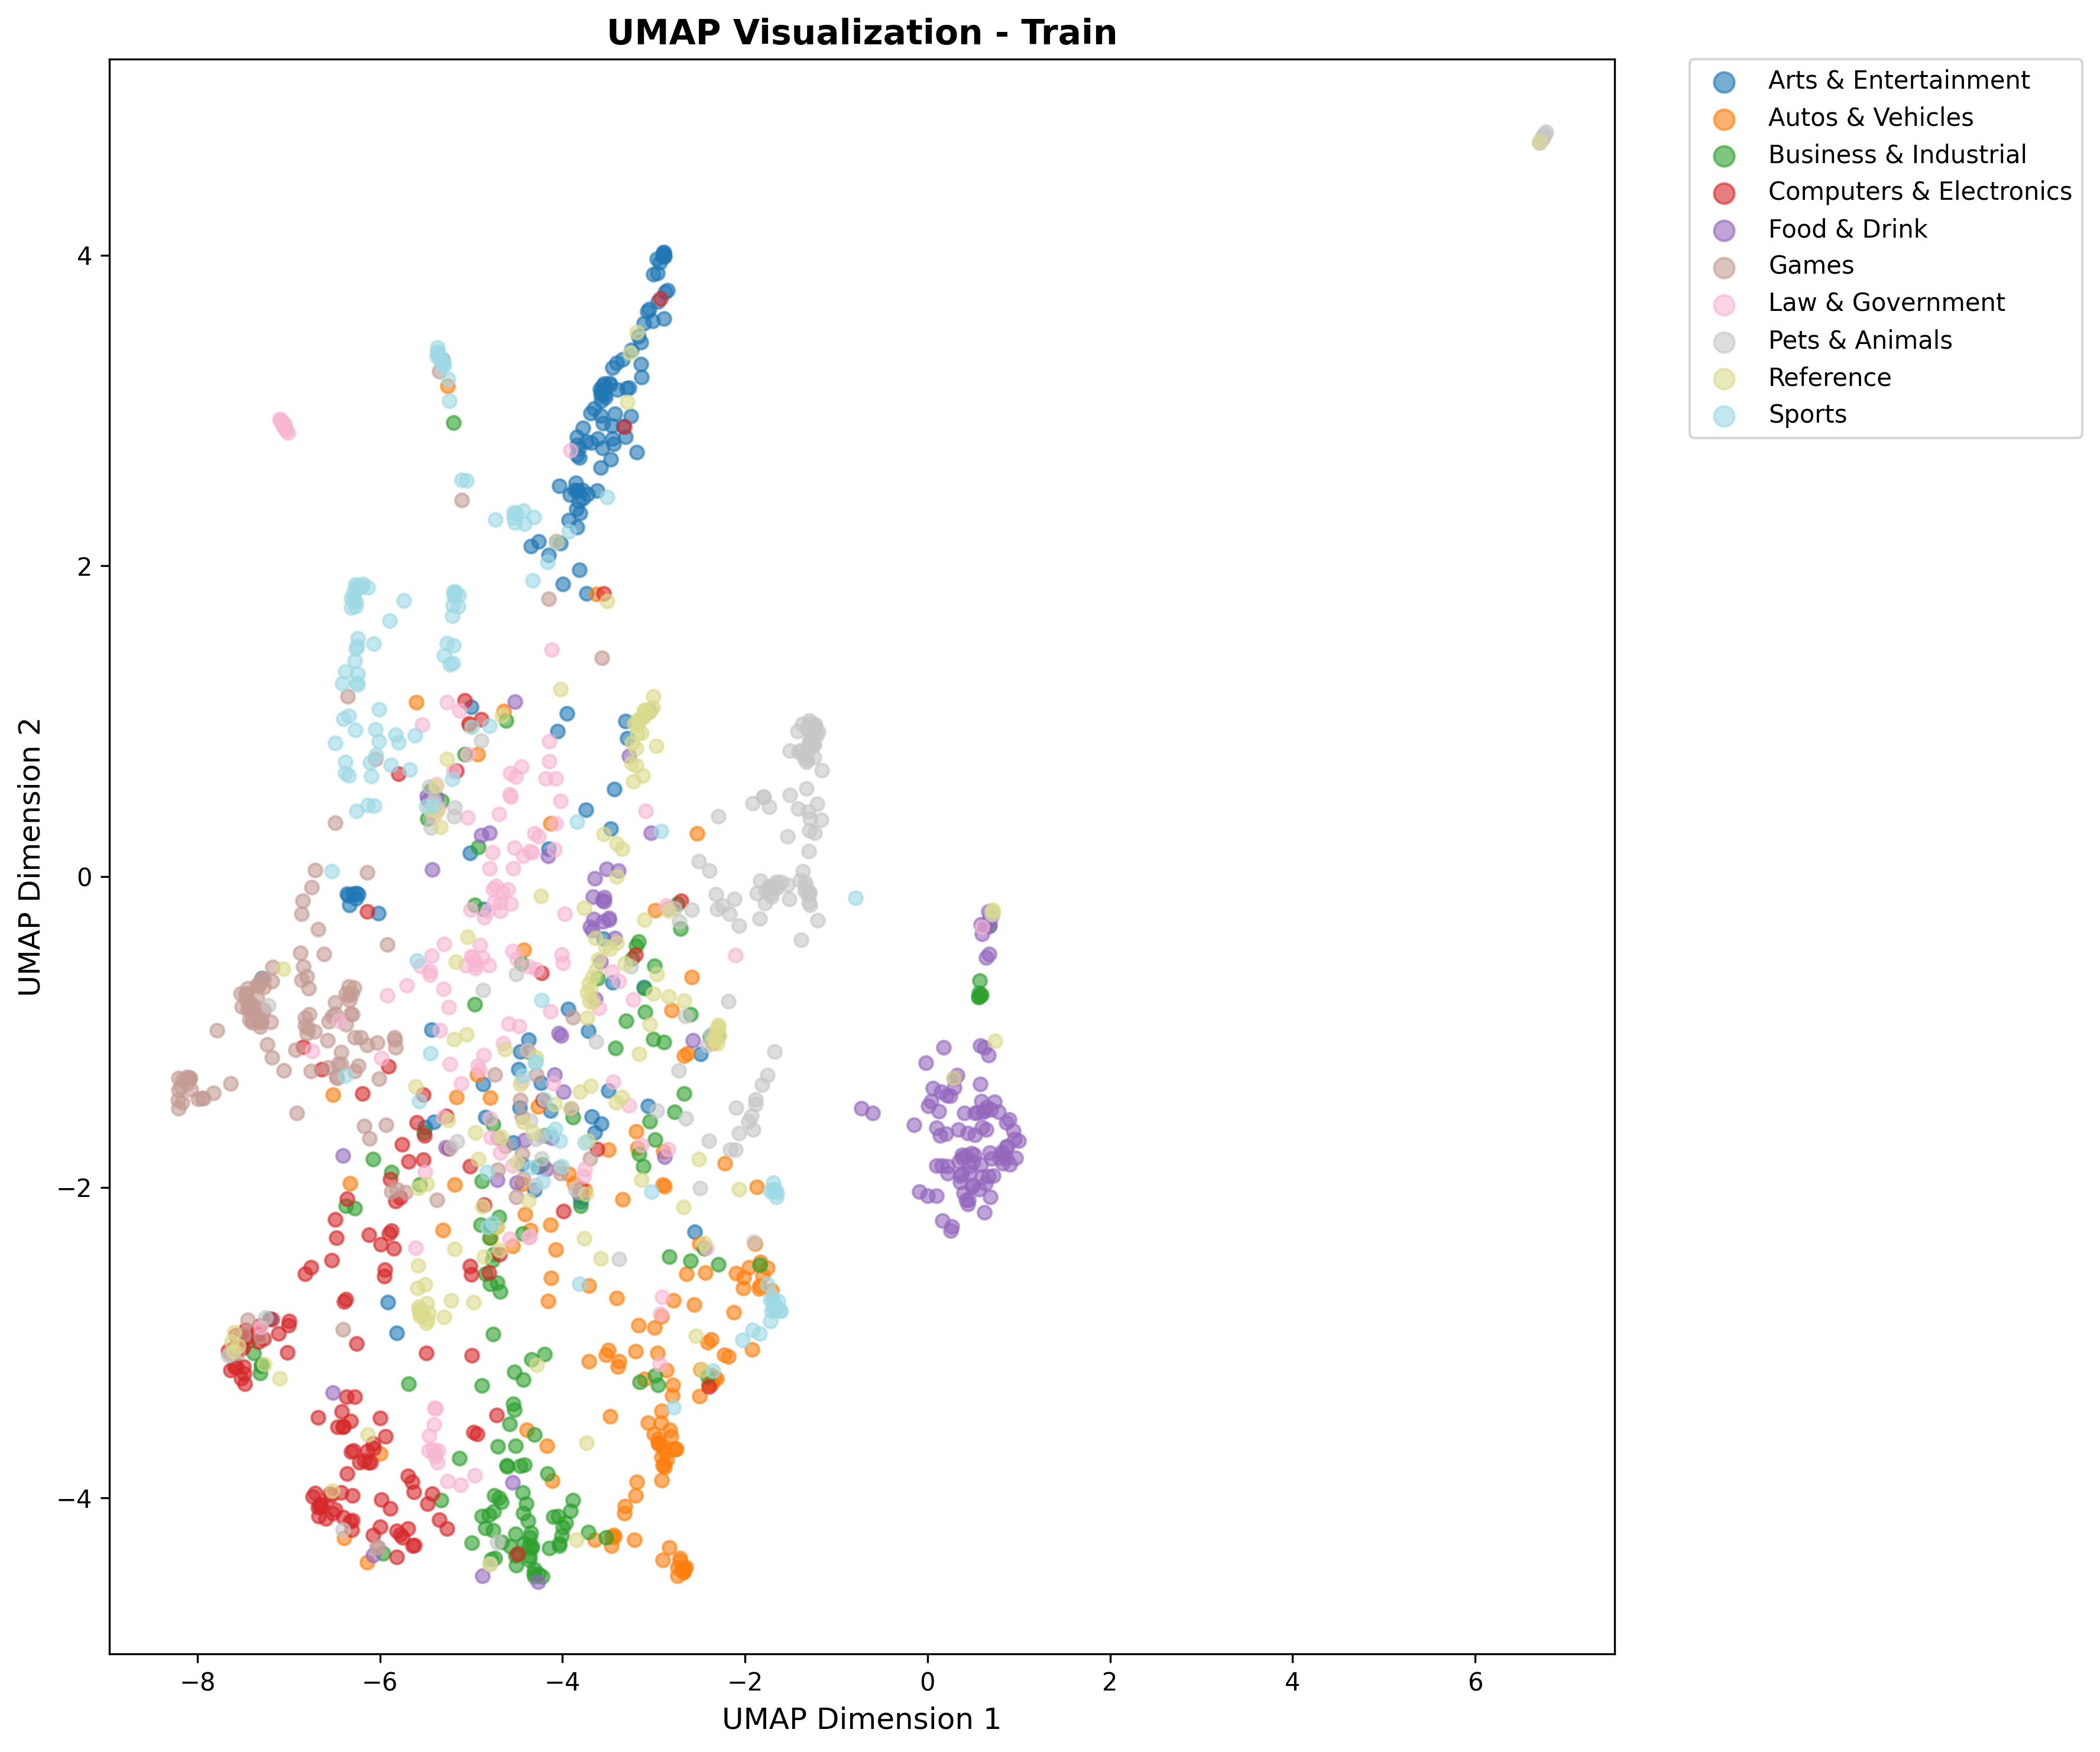
\includegraphics[width=0.8\linewidth]{asset/umap_train.png}
% \end{center}
%    \caption{UMAP visualization of video embeddings from the training set, showing distinct clustering by class.}
% \label{fig:umap}
% \end{figure}


% \subsection{Baseline Models}
% We established two baseline models for comparison:
% \begin{itemize}
%     \item \textbf{Zero-Shot Classification}: Using pre-trained embeddings without any fine-tuning on our dataset, this approach achieved an accuracy of 55.6%[cite: 10, 11].
%     \item \textbf{TimeSformer-Based Classification}: We fine-tuned a TimeSformer model (pre-trained on Kinetics-400\cite{kay2017kinetics}) on our dataset. This model achieved 64.0% accuracy after approximately 10 hours of training[cite: 13].
% \end{itemize}

% \subsection{Proposed Method}
% Our proposed method involves a neural network that takes concatenated multimodal embeddings as input. The architecture consists of a Multi-Layer Perceptron (MLP) followed by a classification layer. Key training parameters include 20 epochs, a batch size of 8, and a CosineAnnealingLR scheduler~\cite{loshchilov2016sgdr}, leading to a total training time of approximately 1 minute.

% \textbf{Data Augmentation}: We introduce a novel data augmentation technique applied directly to the embeddings. Noise is generated, normalized, scaled by an augmentation strength, added to the original embedding, and then the result is re-normalized. This helps to prevent overfitting and improve generalization, particularly in the cosine distance space where these embeddings often operate. 
% % Equation for augmentation could be added here if space allows:
% \[
% noise = strength * gaussian\_noise / ||gaussian\_noise||_2
% \]
% \[
% emb_{aug} = (emb + noise ) / ||emb + noise||_2 
% \]
% The augmentation process is illustrated in Figure~\ref{fig:augmentation}
% \begin{figure}[h]
% \begin{center}
%    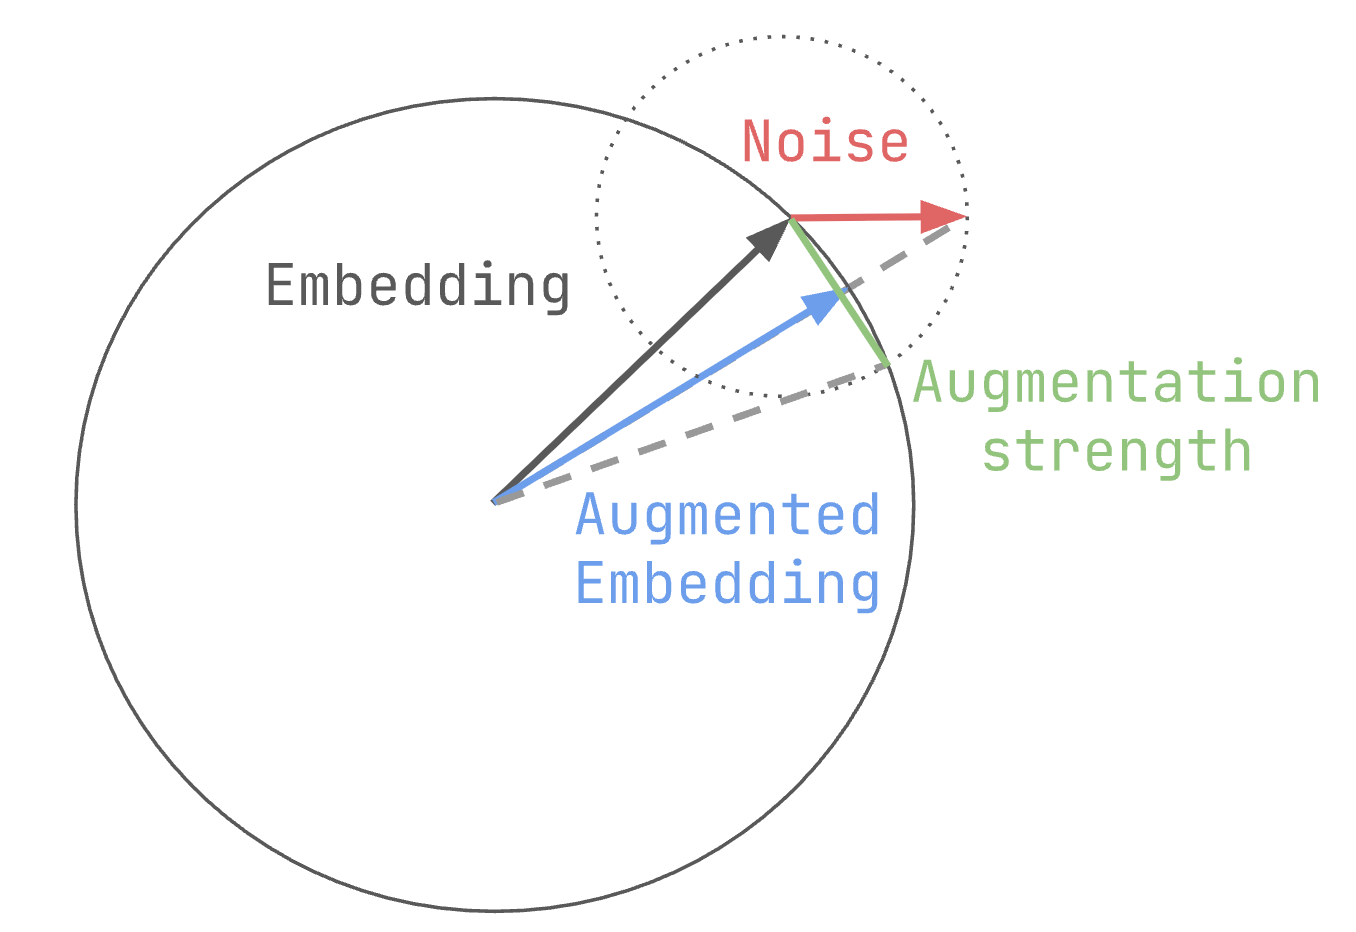
\includegraphics[width=0.8\linewidth]{asset/augmentation.png}
% \end{center}
%    \caption{Data augmentation process on cosine distance space.}
% \label{fig:augmentation}
% \end{figure}


% \section{Methodology}

% \subsection{Dataset and Preprocessing}

% We utilize a subset of the YouTube-8M dataset (May 14, 2018 version)~\cite{abu2016youtube}, comprising approximately 1,800 videos categorized into 10 distinct classes. Each video has an average duration of around 20 seconds. The dataset is divided into training, validation, and test splits using an 8:1:1 ratio.

% Preprocessing involved downloading video shards, sampling the working subset, and extracting various features. For each video, both raw and embedded representations were obtained, including:

% \begin{itemize}
%     \item \textbf{Audio Features}: 1024-dimensional embeddings generated using the TwelveLabs embedding API~\cite{jung2024pegasus, lee2024twlv}.
%     \item \textbf{Video-Text Features}: 1024-dimensional embeddings also produced via the TwelveLabs embedding API~\cite{jung2024pegasus, lee2024twlv}.
%     \item \textbf{Metadata Embeddings}: 3072-dimensional embeddings derived from OpenAI’s \texttt{text-embedding-3-large} model, applied to textual metadata such as video tags.
% \end{itemize}

% All features were serialized into individual HDF5 files to enable efficient loading during training and evaluation. To assess the quality of the embeddings, we employed UMAP~\cite{mcinnes2018umap} for dimensionality reduction. The resulting visualizations, shown in Figure~\ref{fig:umap}, reveal clear class-wise separability.

% \begin{figure}[h]
% \begin{center}
%    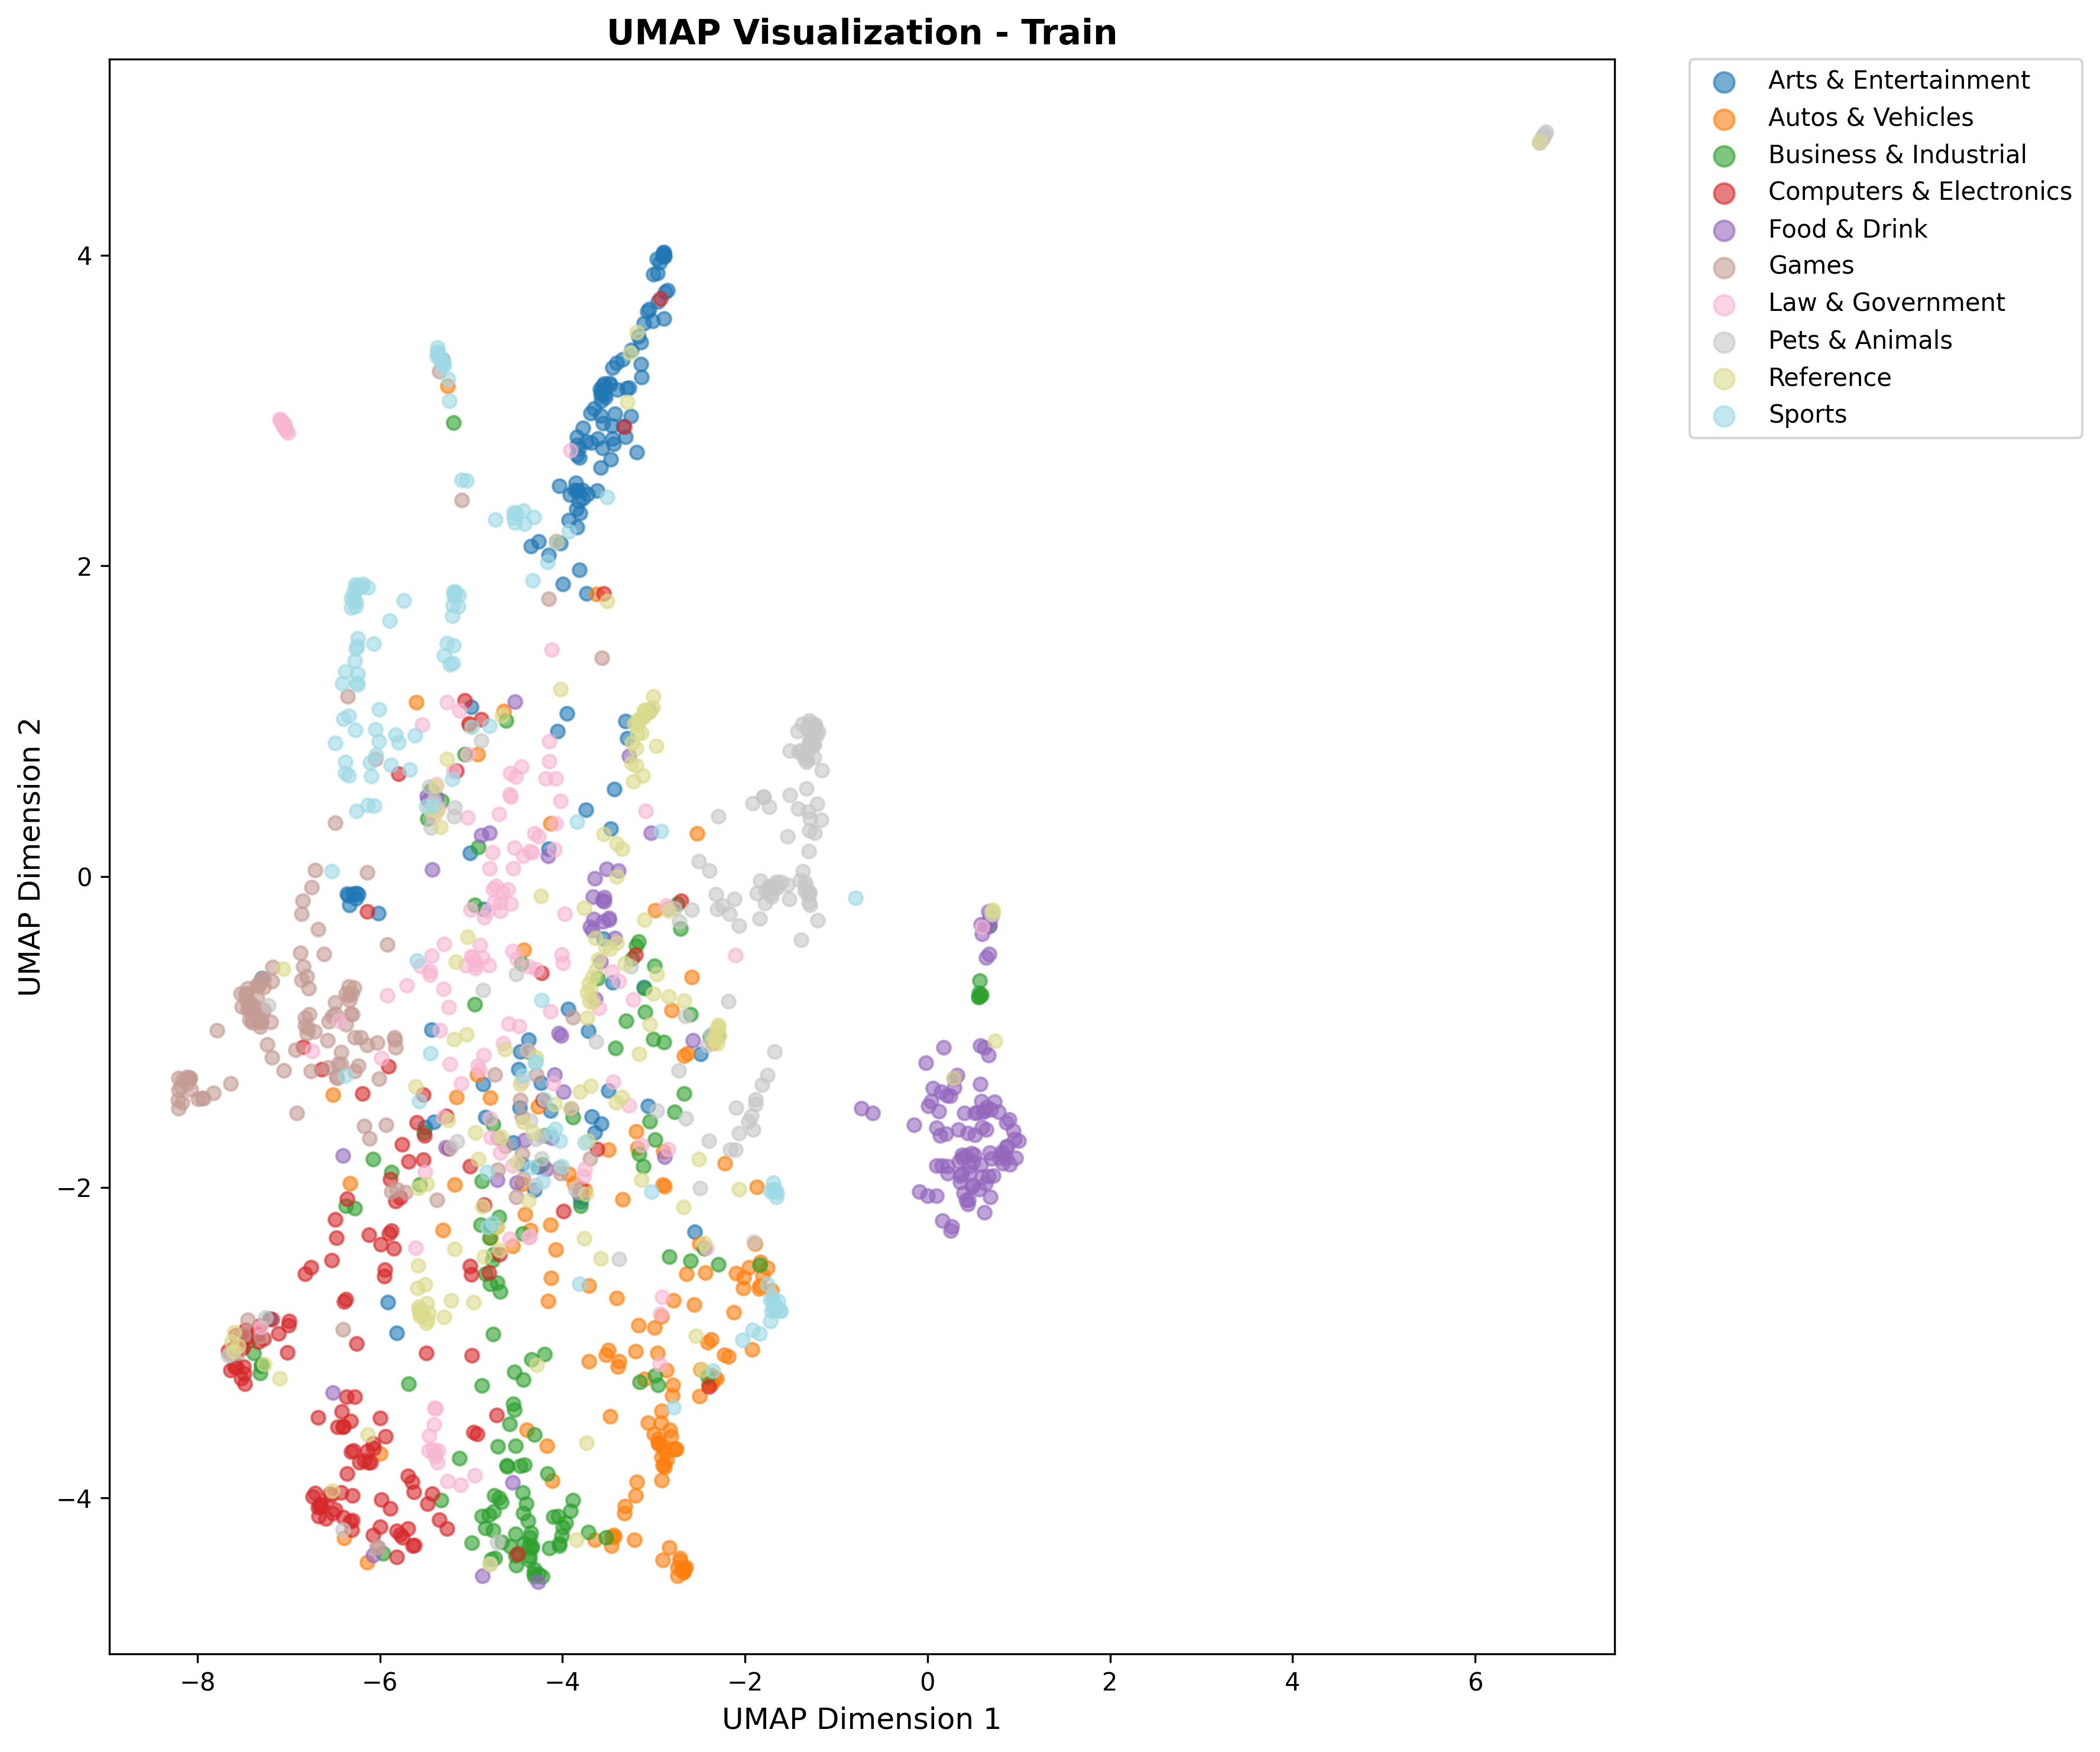
\includegraphics[width=0.8\linewidth]{asset/umap_train.png}
% \end{center}
%    \caption{UMAP visualization of training set video embeddings, illustrating distinct clusters corresponding to different classes.}
% \label{fig:umap}
% \end{figure}

% \subsection{Baseline Models}

% We implemented two baseline models for performance comparison:

% \begin{itemize}
%     \item \textbf{Zero-Shot Classification}: With TwelveLabs video embeddings and text embeddings without any training. It achieved an accuracy of 55.6\%.
    
%     \item \textbf{TimeSformer-Based Classification}: We fine-tuned a TimeSformer model pre-trained on the Kinetics-400 dataset~\cite{kay2017kinetics} using our dataset. This model attained 64.0\% accuracy after approximately 10 hours of training~.
% \end{itemize}

% \subsection{Proposed Method}

% Our proposed model utilizes a neural network that ingests concatenated multimodal embeddings as input. The architecture is composed of a Multi-Layer Perceptron (MLP) followed by a classification head. Key training parameters include 20 epochs, a batch size of 8, and a CosineAnnealingLR scheduler~\cite{loshchilov2016sgdr}, with a total training time of approximately one minute.

% \textbf{Data Augmentation}: To enhance generalization and mitigate overfitting, we introduce a novel augmentation method directly applied to the embeddings. The process involves generating Gaussian noise, normalizing it, scaling it by a configurable strength parameter, adding it to the original embedding, and then re-normalizing the result. This is particularly beneficial in the cosine distance space where these embeddings are typically used.

% The augmentation is defined as:
% \[
% \text{noise} = \text{strength} \times \frac{\text{gaussian\_noise}}{\|\text{gaussian\_noise}\|_2}
% \]
% \[
% \text{emb}_{\text{aug}} = \frac{\text{emb} + \text{noise}}{\|\text{emb} + \text{noise}\|_2}
% \]
% This augmentation process guarantee the augmented embeddings in cosine distance smaller than $1 -  \sqrt{1 - strength ^2}$ with original embedding.
% The augmentation process is illustrated in Figure~\ref{fig:augmentation}.

% \begin{figure}[h]
% \begin{center}
%    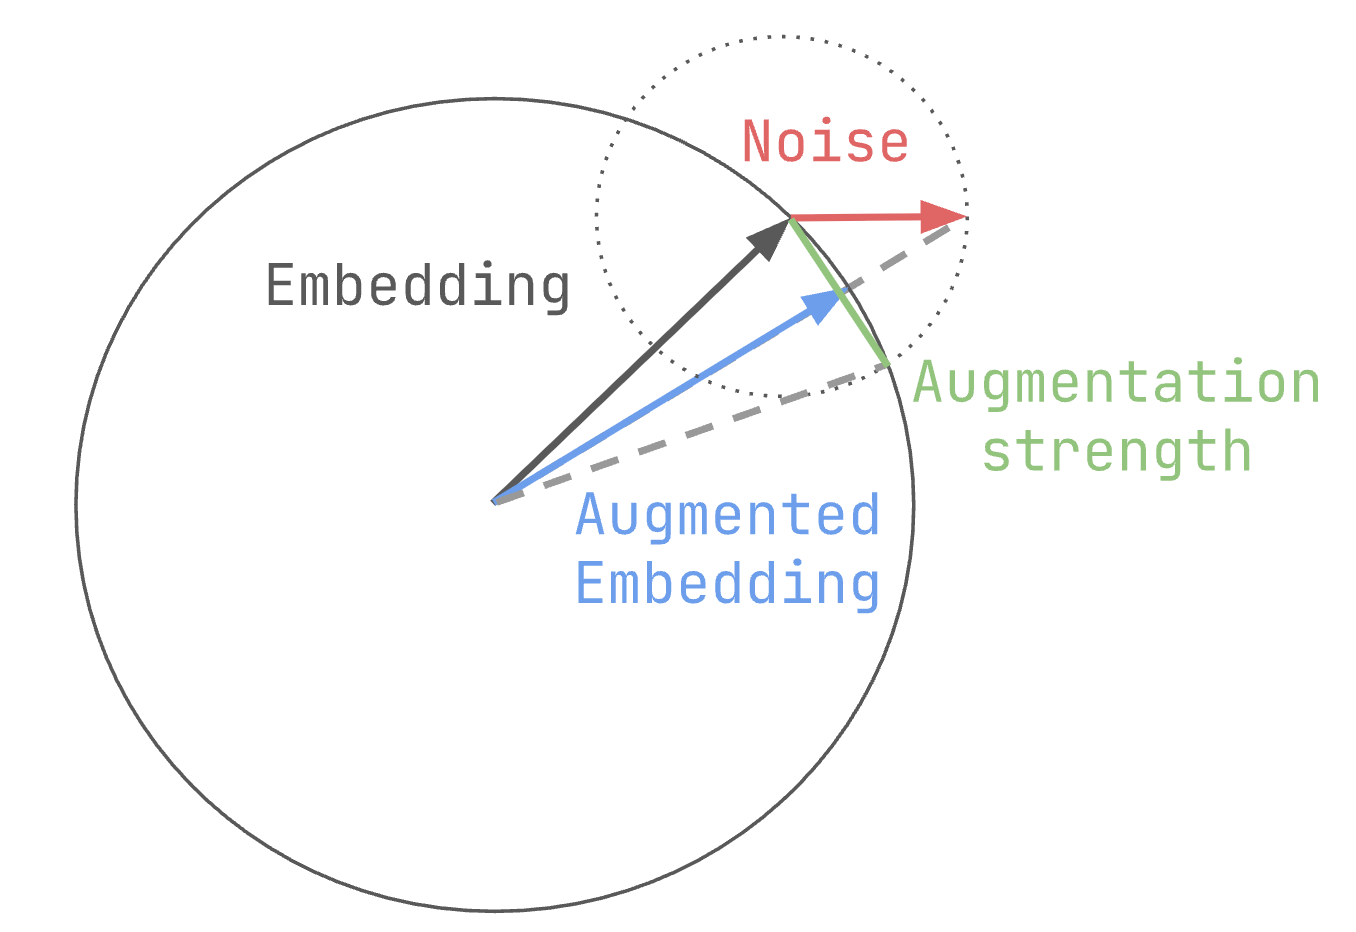
\includegraphics[width=0.8\linewidth]{asset/augmentation.png}
% \end{center}
%    \caption{Illustration of the data augmentation technique in cosine distance space.}
% \label{fig:augmentation}
% \end{figure}

\section{Methodology}

\subsection{Dataset and Preprocessing}

%We use a subset of the YouTube-8M dataset (May 14, 2018 version)~\cite{abu2016youtube}, consisting of approximately 1,800 videos spanning 10 classes. Each video is, on average, about 20 seconds long. We split the data into training, validation, and test sets in an 8:1:1 ratio.

%Preprocessing proceeds as follows:

The present study utilizes a subset of the YouTube-8M dataset (May 14\textsuperscript{th}, 2018 version)~\cite{abu2016youtube}, consisting of approximately 1,800 videos spanning 10 classes: \textit{Arts \& Entertainment}, \textit{Autos \& Vehicles}, \textit{Business \& Industrial}, \textit{Computers \& Electronics}, \textit{Food \& Drink}, \textit{Games}, \textit{Law \& Government}, \textit{Pets \& Animals}, \textit{Reference}, and \textit{Sports}.
The duration of each video is approximately 20 seconds on average.
The data was then divided into training, validation and test sets in an 8:1:1 ratio.

The preprocessing procedure is outlined as follows:

%\begin{enumerate}
    %\item Download the full YouTube-8M video shards.
    %\item Sample the working subset of 1,800 videos (balanced across the 10 classes).
    %\item For each video, extract and save:
    %\begin{itemize}
        %\item \textbf{Audio Embeddings}: 1,024-dimensional vectors via the TwelveLabs embedding API~\cite{jung2024pegasus, lee2024twlv}.
        %\item \textbf{Video–Text Embeddings}: 1,024-dimensional vectors via the TwelveLabs embedding API~\cite{jung2024pegasus, lee2024twlv}.
        %\item \textbf{Metadata Embeddings}: 3,072-dimensional vectors computed by applying %OpenAI’s \texttt{text-embedding-3-large} model~\cite{openai_text_embedding_3_large} to textual metadata (e.g., video tags).
    %\end{itemize}
    %\item Serialize all embeddings into individual HDF5 files for efficient loading during %training and evaluation.
%\end{enumerate}

\begin{enumerate}
    \item YouTube-8M dataset video shards are downloaded.
    \item The working subset of 1,800 videos, balanced across the 10 classes, is sampled.
    \item For each video, the following embeddings are extracted:
    \begin{itemize}
        \item \textbf{Video\-Text and Audio Embeddings}: The TwelveLabs embedding API~\cite{lee2024twlv, twelvelabs_embed_api_doc} facilitates the extraction of 1,024-dimensional vectors.
        \item \textbf{Metadata Embeddings}: A total of 3,072-dimensional vectors have been computed by applying OpenAI's \texttt{text-embedding-3-large} model~\cite{openai_text_embedding_3_large} to textual metadata, such as video tags.
    \end{itemize}
    \item All embeddings are serialized into individual HDF5 files, thus ensuring efficient loading during the training and evaluation phases.
\end{enumerate}

%To verify that the pretrained embeddings exhibit class-wise structure, we apply UMAP~\cite{mcinnes2018umap} to reduce the dimensionality of the video–text embeddings. As shown in Figure~\ref{fig:umap}, the resulting 2D projection reveals clear clusters corresponding to different classes.

Videos are additionally processed to meet the resolution and aspect ratio requirements defined by the TwelveLabs Embed API.
Specifically, a Python module leveraging the MoviePy library assesses each video's original resolution and aspect ratio, resizing and padding the videos to align with the nearest allowed dimensions (e.g., 1:1, 4:3, 16:9).
This ensures all videos consistently meet API specifications, streamlining the embedding extraction process.

To verify that the pretrained embeddings exhibit class-wise structure, the Unsupervised Manifold Alignment Projection (UMAP)~\cite{mcinnes2018umap} algorithm is applied to reduce the dimensionality of the video-text embeddings.
As demonstrated in Figure~\ref{fig:umap}, the resulting 2D projection reveals distinct clusters corresponding to different classes.

\begin{figure}[h]
\centering
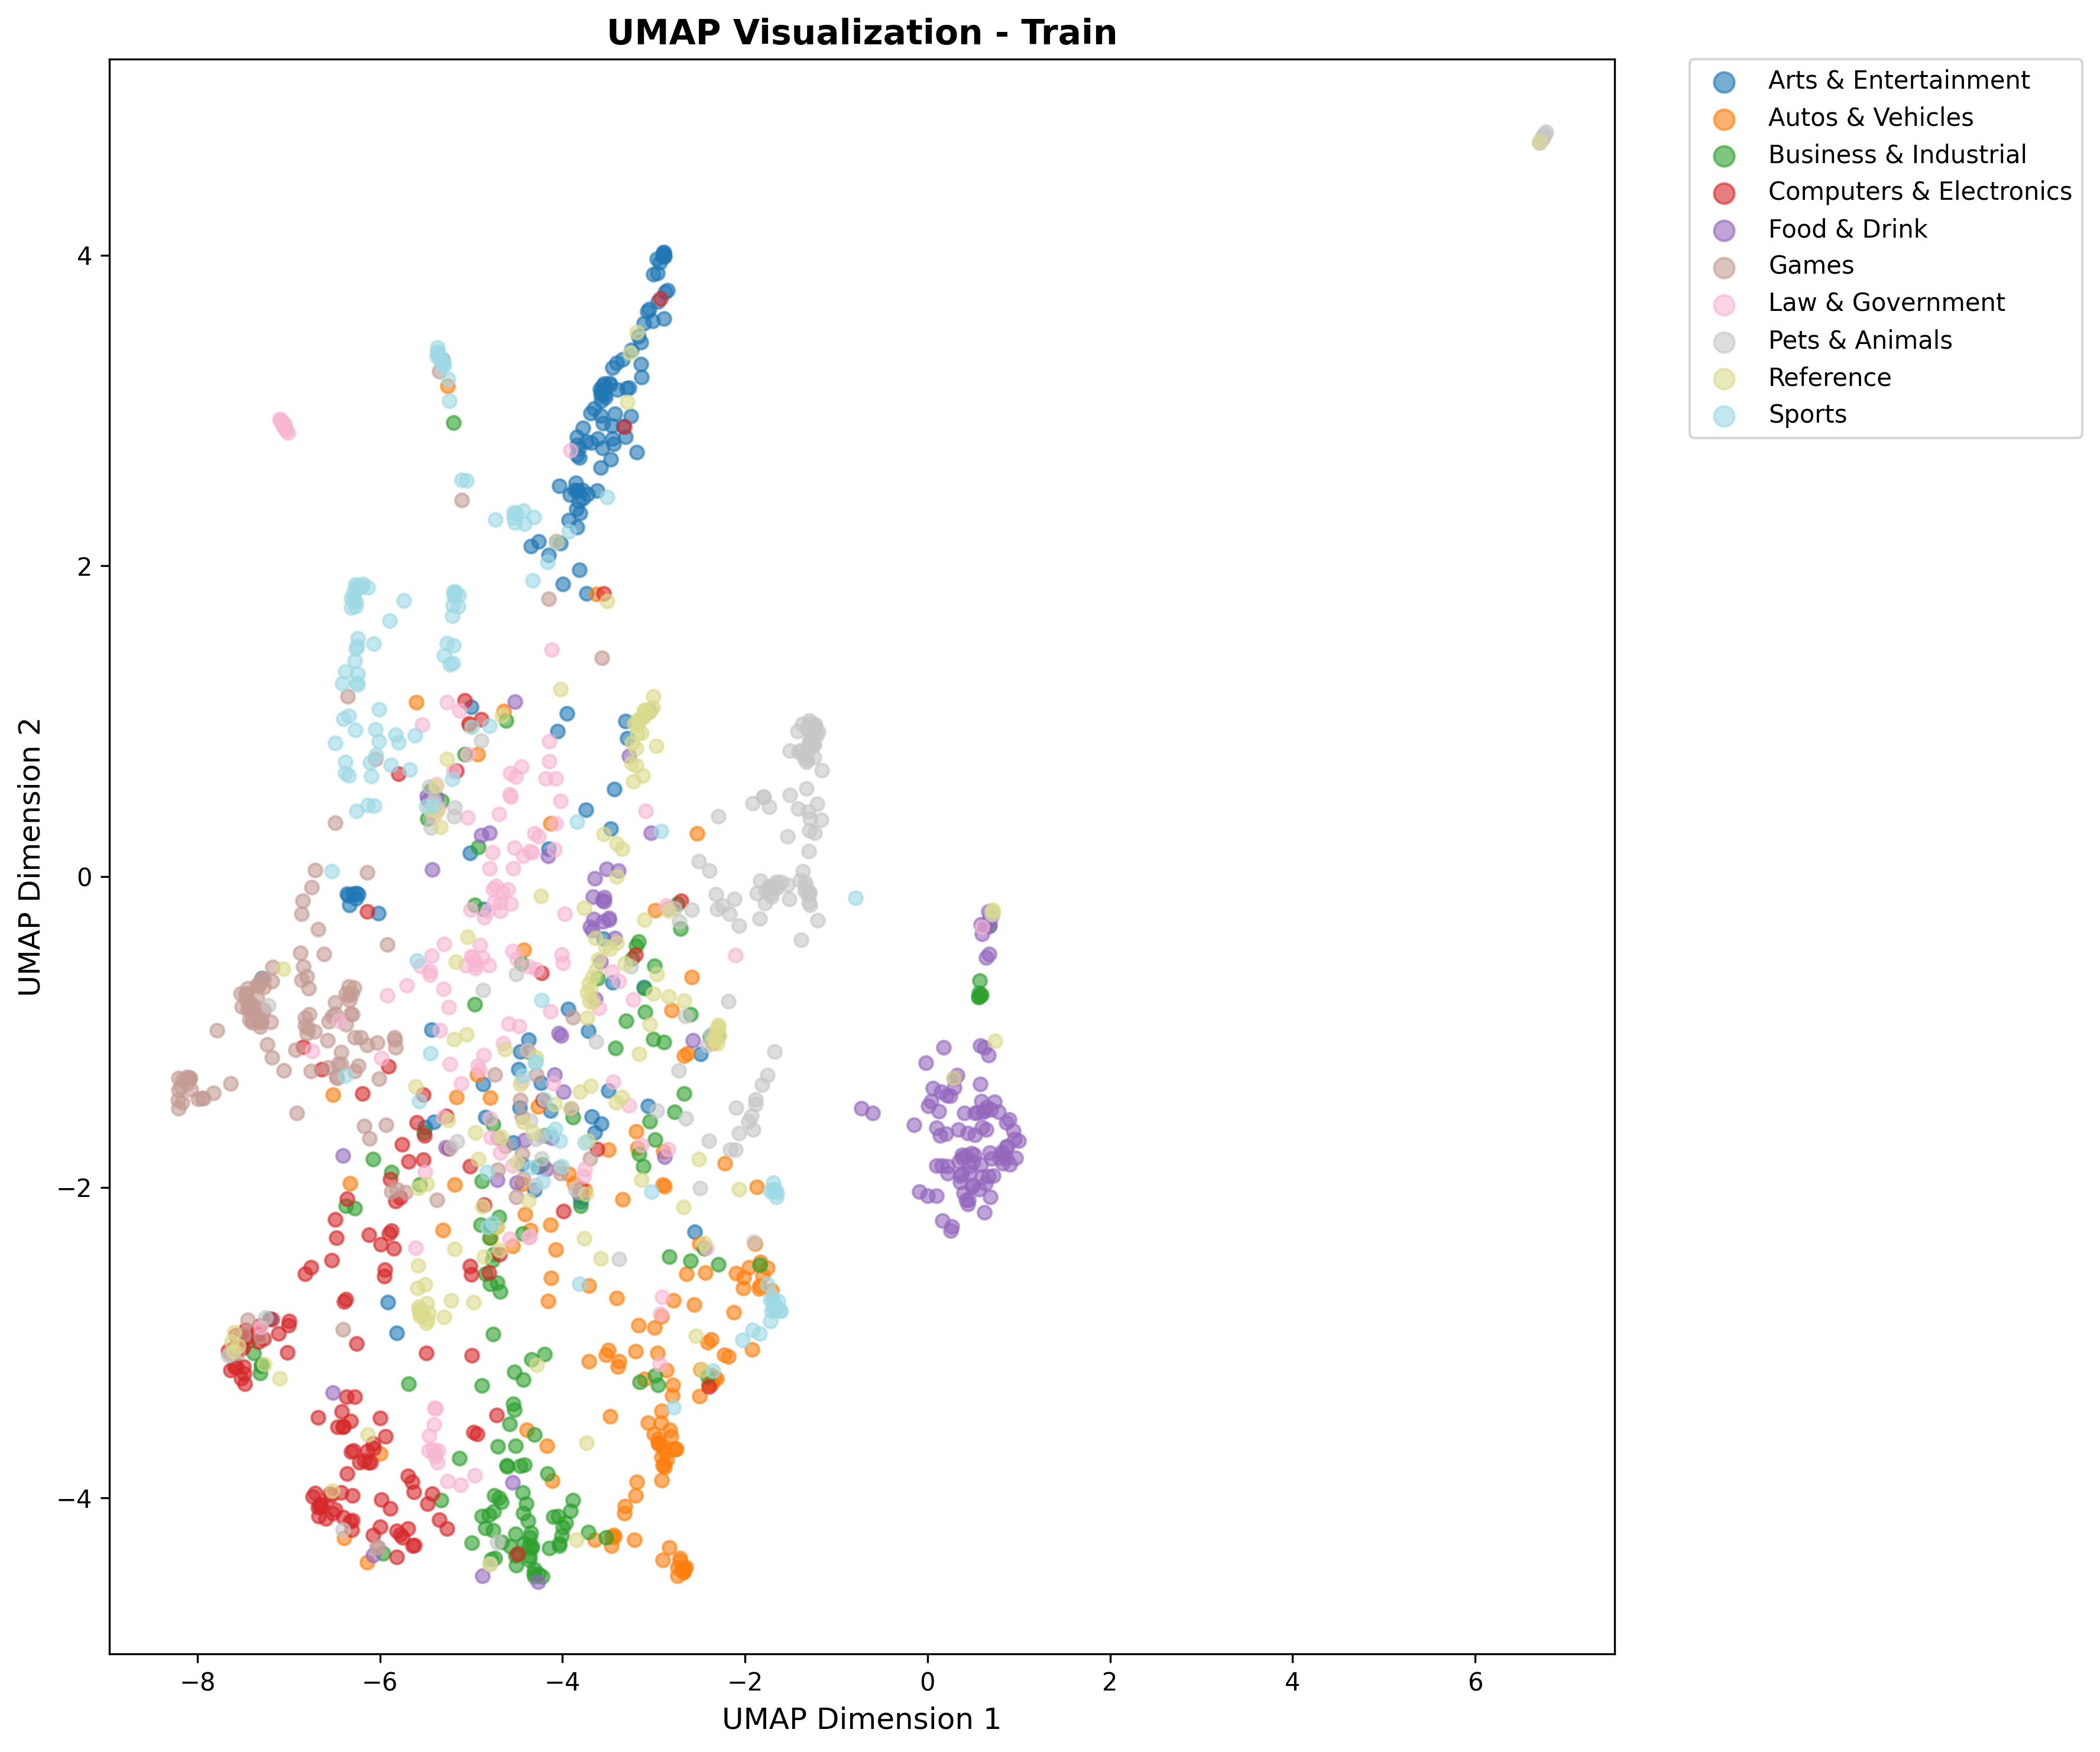
\includegraphics[width=0.8\linewidth]{asset/umap_train.png}
\caption{UMAP projection of video–text embeddings from the training set, illustrating distinct clusters for each class.}
\label{fig:umap}
\end{figure}

\subsection{Baseline Models}

%We implement two baselines for comparison:

Two baselines are implemented for the purpose of comparison:

%\begin{itemize}
    %\item \textbf{Zero-Shot Classification}: We feed the precomputed TwelveLabs video–text and text embeddings directly into a nearest-neighbor classification scheme, without any task-specific training. This approach achieves 55.6\% accuracy.
    
    %\item \textbf{TimeSformer Fine-Tuning}: We fine-tune a TimeSformer model pre-trained on Kinetics-400~\cite{kay2017kinetics} using our 1,800-video subset. After approximately 10 hours of training, this model reaches 64.0\% accuracy.
%\end{itemize}

\begin{itemize}
    \item \textbf{Zero-Shot Classification}: The precomputed TwelveLabs video-text and text embeddings are directly fed into a nearest-neighbor classification scheme, without the necessity for any task-specific training. This approach has been demonstrated to achieve an accuracy of 55.6\%.
    \item \textbf{TimeSformer Fine-Tuning}: The TimeSformer model, which has been pre-trained on Kinetics-400, is fine-tuned using a subset of 1,800 videos. Following a training period of approximately 10 hours, the model attains an accuracy of 64.0\%.
\end{itemize}

\subsection{Proposed Method}

%Our model concatenates the multimodal embeddings for each video and feeds them into a lightweight neural network consisting of:

The proposed model integrates the multimodal embeddings for each video, subsequently inputting them into a lightweight neural network comprising the following components:

%\begin{itemize}
    %\item An input layer that accepts the concatenated vector.
    %\item A Multi-Layer Perceptron (MLP) with four hidden layers (each followed by Swish activations, batch normalization, and dropout).
    %\item A final linear classification head that outputs logits over the 10 classes.
%\end{itemize}

\begin{itemize}
    \item The input layer is responsible for accepting the concatenated vector.
    \item The Multi-Layer Perceptron (MLP) layer, with four hidden layers, each of which is followed by Swish activations, batch normalization, and dropout.
    \item The final linear classification head, which generates logits for the 10 classes.
\end{itemize}

%We train for 20 epochs with a batch size of 8, using the AdamW optimizer and a CosineAnnealingLR scheduler~\cite{loshchilov2016sgdr}. On our hardware setup, total training time is approximately one minute.

The training process is conducted over a total of 20 epochs, with a batch size of 8.
The AdamW optimizer and a CosineAnnealingLR scheduler~\cite{loshchilov2016sgdr} are employed to ensure the efficient convergence of the model parameters.
The total duration of training on our hardware configuration is estimated to be approximately one minute.

%\paragraph{Embedding-Space Augmentation} To improve generalization and reduce overfitting, we apply a novel augmentation directly in embedding space. For each original embedding $\mathbf{e}$, we generate a perturbed version as follows:

\paragraph{Embedding-Space Augmentation} To enhance the generalization capabilities and mitigate the risk of overfitting, a novel augmentation technique is employed directly within the embedding space.
For each original embedding, denoted by $\mathbf{e}$, a perturbed version is generated according to the following method.
\[
\mathbf{n} = \frac{\boldsymbol{\epsilon}}{\|\boldsymbol{\epsilon}\|_2}, \quad
\boldsymbol{\epsilon} \sim \mathcal{N}(\mathbf{0},\,\mathbf{I}),
\]
\[
\mathbf{n}_{\text{scaled}} = \alpha \,\mathbf{n},\quad
\widetilde{\mathbf{e}} = \frac{\mathbf{e} + \mathbf{n}_{\text{scaled}}}{\|\mathbf{e} + \mathbf{n}_{\text{scaled}}\|_2},
\]
where \(\alpha\) is a user-defined \emph{strength} parameter. This procedure ensures that the cosine distance between \(\widetilde{\mathbf{e}}\) and \(\mathbf{e}\) is at most 
\[
1 - \sqrt{1 - \alpha^2}.
\]

%Applying Gaussian noise in this normalized way preserves the overall magnitude of the embedding while encouraging robustness to small perturbations in cosine space. Figure~\ref{fig:augmentation} illustrates the augmentation process.

The application of Gaussian noise in this normalized manner preserves the magnitude of the embedding in its entirety whilst encouraging robustness to minor perturbations in cosine space. As demonstrated in Figure~\ref{fig:augmentation}, the augmentation process is illustrated.

\begin{figure}[h]
\centering
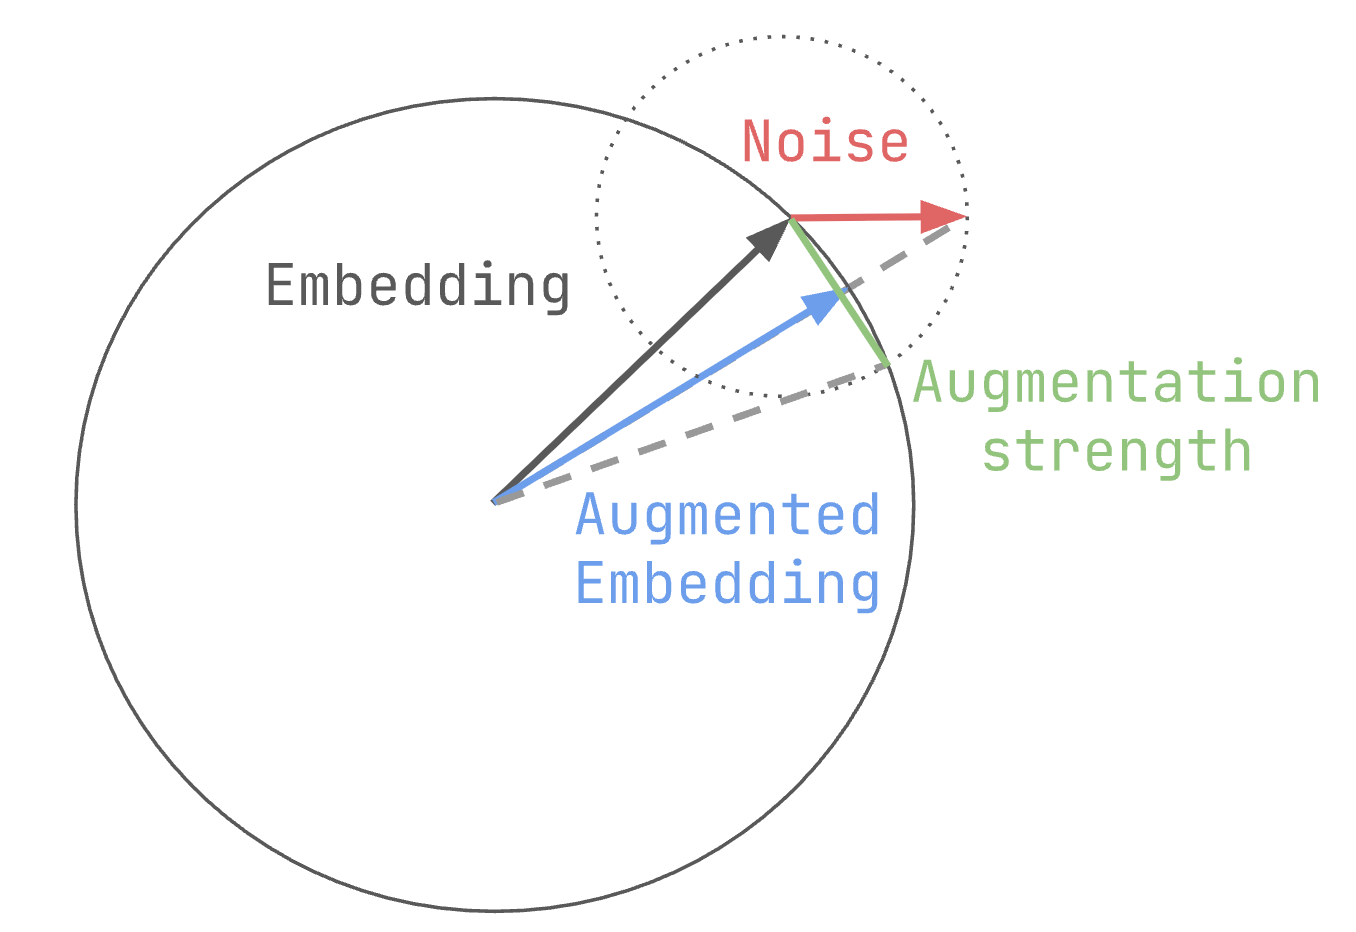
\includegraphics[width=0.6\linewidth]{asset/augmentation.png}
\caption{Schematic of the embedding-space augmentation: Gaussian noise is normalized, scaled by \(\alpha\), added to the original embedding, and then re-normalized.}
\label{fig:augmentation}
\end{figure}
\vspace{-10pt}
\section{Experiments}

%We conducted extensive ablation studies to evaluate the contribution of each component of our proposed method. We emphasize validation loss for model selection due to the relatively small validation set size (180 videos), which can make accuracy metrics noisy.

Extensive ablation studies were conducted to evaluate the contribution of each component of the proposed method.
The emphasis placed on validation loss for model selection is due to the relatively small size of the validation set (180 videos), which can render accuracy metrics unreliable.

\subsection{Implementation Details}

%For our proposed model, we utilized a Multi-Layer Perceptron (MLP) architecture. The input to the MLP was formed by concatenating pre-extracted video, audio (from TwelveLabs models), and string metadata embeddings (from OpenAI models). Based on our ablation studies, the optimal architecture was a 4-layer MLP with Swish~\cite{hendrycks2016gaussian} activation functions, dropout layer and batch normalization layer in the hidden layers and a final softmax layer for classification across the 10 categories.

%The model was trained for 20 epochs with a batch size of 8. We employed the AdamW~\cite{loshchilov2017decoupled} optimizer and a Cosine Annealing learning rate scheduler with a peak learning rate of $1\times 10^{-4}$ and a linear warm-up period of 1 epoch. The standard cross-entropy loss function was used for training. Data augmentation, with a strength of 0.5 as determined by our ablation studies, was applied to the input embeddings during training.

For the proposed model, an MLP architecture was utilized.
The input was formed by concatenating pre-extracted video, audio (from TwelveLabs models), and string metadata embeddings (from OpenAI models).
Considering the findings from the ablation experiments, it can be concluded that the most effective architecture is a 4-layer MLP with Swish ~\cite{hendrycks2016gaussian} activation functions, a dropout layer, batch normalization layers within the hidden layers and a final softmax layer, for the classification across the 10 distinct categories.
The model was trained over a period of 20 epochs, with a batch size of 8.
The AdamW ~\cite{loshchilov2017decoupled} optimizer and a Cosine Annealing learning rate scheduler with a peak learning rate of $1\times 10^{-4}$ and a linear warm-up period of 1 epoch were employed.
The standard cross-entropy loss function was utilized for the training process.
The augmentation of data, with a strength of 0.5 as determined by our ablation studies, was applied to the input embeddings during the training process.

\subsection{Ablation Studies}

\subsubsection{Input Features}

%Our ablation study on input features revealed clear benefits to incorporating multimodal information alongside basic video embeddings. While adding audio embeddings to the video embeddings offered a modest performance increase, the inclusion of metadata embeddings provided the most substantial improvement in validation accuracy. Interestingly, combining all three embedding types (video, audio, and metadata) did not yield the best accuracy and also showed signs of potential overfitting, as indicated by its validation loss trend. Considering both the significant accuracy uplift and a stable validation loss profile, the combination of video and metadata embeddings emerged as the most effective and was selected for subsequent experiments.

This study has revealed the clear benefits of incorporating multimodal information alongside basic video embeddings.
While the incorporation of audio embeddings into the video embeddings resulted in a modest enhancement to performance, the integration of metadata embeddings yielded the most substantial enhancement in validation accuracy.
It is interesting to note that combining all three embedding types (video, audio, and metadata) did not result in the optimal level of accuracy and exhibited signs of potential overfitting, as indicated by its validation loss trend.
Based on a comprehensive evaluation encompassing both the substantial enhancement in accuracy and the consistent stability of validation loss profiles, the integration of video and metadata embeddings was identified as the most effective approach.
Consequently, this combination was selected for further experiments.

\begin{table}[hbt!]
\centering
\caption{Ablation Study on Input Features. Validation accuracy is reported.}
\label{tab:input_ablation}
\small % Use \small or \footnotesize if needed for space
\begin{tabular}{lc}
\toprule
Input Features Combination & Valid. Accuracy (\%) \\
\midrule
Video Embedding Only & 72.8 \\
+ Audio Embedding  & 73.9 \\
\textbf{+ Metadata Embedding} & \textbf{81.1} \\
+ All Embeddings& 79.4 \\
\bottomrule
\end{tabular}
\end{table}

\subsubsection{Data Augmentation Strength}

%We investigated the optimal augmentation strength for both video and metadata embeddings. For video embeddings, a strength of 0.5 consistently yielded the best performance across both validation loss and accuracy. This suggests a clear optimal point for introducing noise to the video features.

%In the case of metadata embeddings, the results presented a slightly more nuanced scenario. While a higher augmentation strength of 1.0 led to a marginally better peak validation accuracy, an augmentation strength of 0.5 demonstrated superior stability in its validation loss profile. Given our small validation set and the potential for noisy accuracy readings, we prioritized the more stable generalization indicated by the validation loss. Therefore, an augmentation strength of 0.5 was selected for metadata embeddings as well, aiming for a robust and reliable improvement.

The study investigated the optimal augmentation strength for both video and metadata embeddings.
In the context of video embeddings, a strength of 0.5 has been shown to consistently yield optimal performance across both validation loss and accuracy.
This finding indicates a clear optimal point for introducing noise to the video features.

In the case of metadata embeddings, the results presented a slightly more nuanced scenario.
While an augmentation strength of 1.0 led to a marginally superior peak validation accuracy, an augmentation strength of 0.5 demonstrated superior stability in its validation loss profile.
Given the limited size of the validation set and the possibility of inaccurate accuracy readings, the more stable generalization indicated by the validation loss was given priority.
Consequently, an augmentation strength of 0.5 was selected for metadata embeddings as well, with the objective of achieving a robust and reliable improvement.

\begin{table}[hbt!]
\centering
\caption{Ablation Study on Video Embedding Augmentation Strength. Validation accuracy is reported.}
\label{tab:video_aug_ablation}
\small
\begin{tabular}{lc}
\toprule
Augmentation Strength & Valid. Accuracy (\%) \\
\midrule
Video Embedding & 72.8 \\
+ 0.01 Aug. Strength & 72.2 \\
+ 0.05 Aug. Strength  & 72.8 \\
+ 0.1 Aug. Strength & 73.3 \\
\textbf{+ 0.5 Aug. Strength} & \textbf{75.0} \\
+ 1.0 Aug. Strength & 70.0 \\
\bottomrule
\end{tabular}
\end{table}

\begin{table}[hbt!]
\centering
\caption{Ablation Study on Metadata Embedding Augmentation Strength. The baseline is Video + Metadata embeddings without metadata augmentation. Validation accuracy is reported.}
\label{tab:metadata_aug_ablation}
\small
\begin{tabular}{lc}
\toprule
Augmentation Strength (on Metadata) & Valid. Accuracy (\%) \\
\midrule
Video emb. \& Metadata emb & 81.1 \\
+ 0.1 Aug. Strength & 80.0 \\
+ 0.5 Aug. Strength & 80.0 \\
\textbf{+ 1.0 Aug. Strength} & \textbf{82.2} \\
\bottomrule
\end{tabular}
\end{table}

\subsubsection{Model Architecture}

%To determine the optimal model structure, we experimented with Multi-Layer Perceptrons (MLPs) of varying depths and an attention-based model, keeping the data augmentation strength fixed at 0.5. Our findings, detailed in Table~\ref{tab:arch_ablation}, indicate that a 4-layer MLP achieved the highest validation accuracy. Increasing the depth to a 5-layer MLP led to a decline in performance, suggesting that deeper models were prone to overfitting with our dataset size and feature complexity. The attention-based model, which incorporated a 1D self-attention mechanism, yielded a competitive accuracy and notably demonstrated good generalization as evidenced by its stable validation loss curve. However, it did not surpass the peak accuracy of the 4-layer MLP. Consequently, the 4-layer MLP was selected as the optimal architecture for our proposed method due to its superior accuracy.

To determine the optimal model structure, experiments were conducted with MLP of varying depths and an attention-based model, whilst maintaining the data augmentation strength at 0.5.
The findings, which are outlined in Table~\ref{tab:arch_ablation}, indicate that a 4-layer MLP achieved the maximum validation accuracy.
Increasing the depth to a 5-layer MLP led to a decline in performance, suggesting that deeper models were prone to overfitting with the size of the dataset and the complexity of the features.
The attention-based model, incorporating a 1D self-attention mechanism, demonstrated competitive accuracy and notably exhibited good generalization, as evidenced by its stable validation loss curve.
However, this configuration did not exceed the peak accuracy of the 4-layer MLP.
Consequently, the latter one was selected as the optimal architecture for the proposed method due to its superior accuracy.

\begin{table}[hbt!]
\centering
\caption{Ablation Study on Model Architecture. Validation accuracy is reported.}
\label{tab:arch_ablation}
\small
\begin{tabular}{lc}
\toprule
Model Architecture & Valid. Accuracy (\%) \\
\midrule
3 layers (MLP)  & 80.6  \\
\textbf{4 layers (MLP)} & \textbf{81.1} \\
5 layers (MLP) & 78.3 \\
Attention & 79.4 \\
\bottomrule
\end{tabular}
\end{table}

\subsection{Overall Performance}

%Our final model, incorporating video and metadata embeddings, 0.5 augmentation strength, and a 4-layer MLP, demonstrates significant improvements over the baselines. The progression of validation accuracy is summarized in Figure~\ref{fig:summary_results} . The test set confusion matrix for this model is shown in Figure~\ref{fig:confusion_matrix}.

The final model, incorporating video and metadata embeddings, 0.5 augmentation strength, and a 4-layer MLP, demonstrates significant improvements over the baselines.
% The progression of validation accuracy is summarized in Figure ~\ref{fig:summary_results}, while the test set confusion matrix for this model is shown in Figure~\ref{fig:confusion_matrix}.
The test set confusion matrix for this model is shown in Figure~\ref{fig:confusion_matrix}.

% Placeholder for summary results figure
% \begin{figure}[t]
% \begin{center}
% % \fbox{\rule{0pt}{2in} \rule{0.9\linewidth}{0pt}}
%    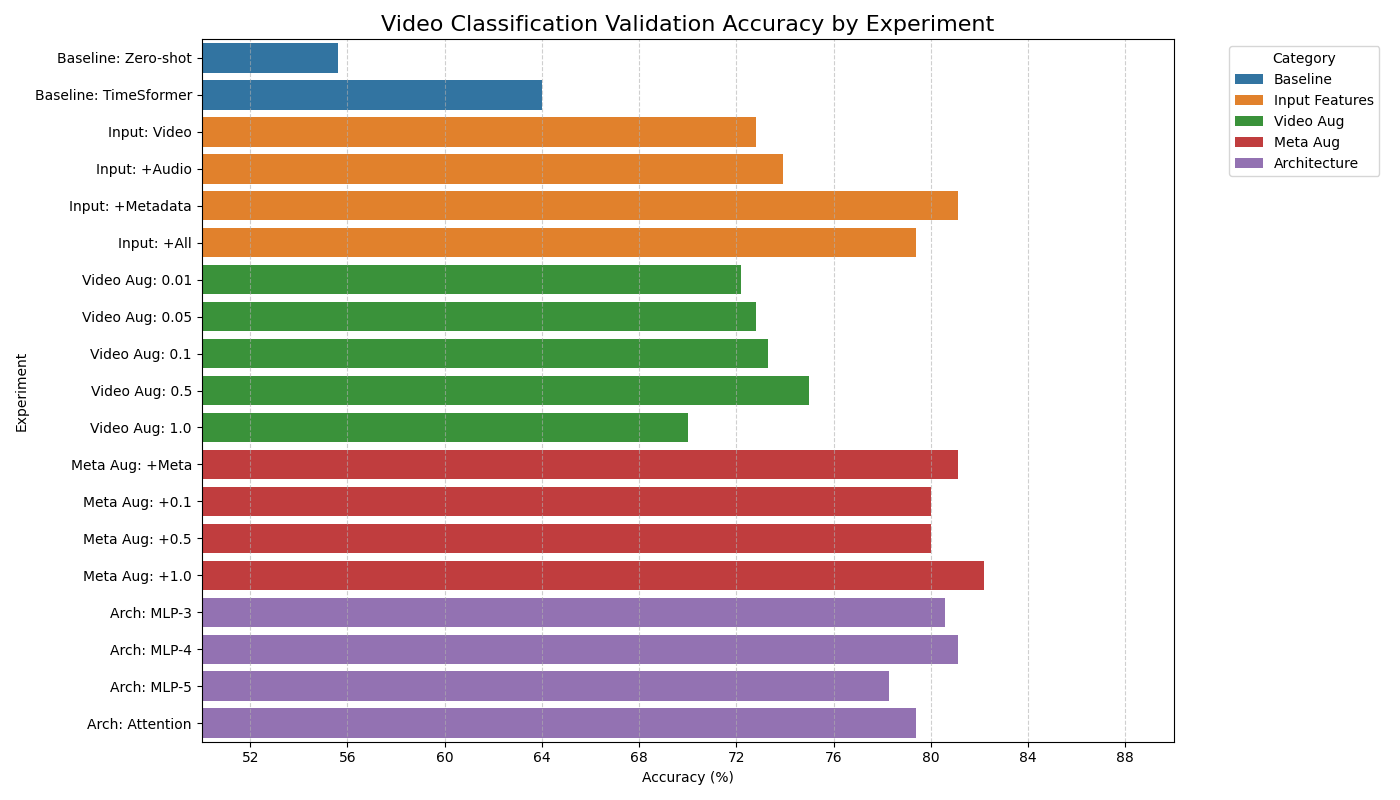
\includegraphics[width=0.8\linewidth]{asset/accuracy_plot.png} % Replace with actual image
% \end{center}
%    \caption{Summary of validation accuracy by experiment, showing progressive improvements.}
% \label{fig:summary_results}
% \end{figure}

% Placeholder for confusion matrix
\begin{figure}[t]
\begin{center}
% \fbox{\rule{0pt}{2in} \rule{0.9\linewidth}{0pt}}
   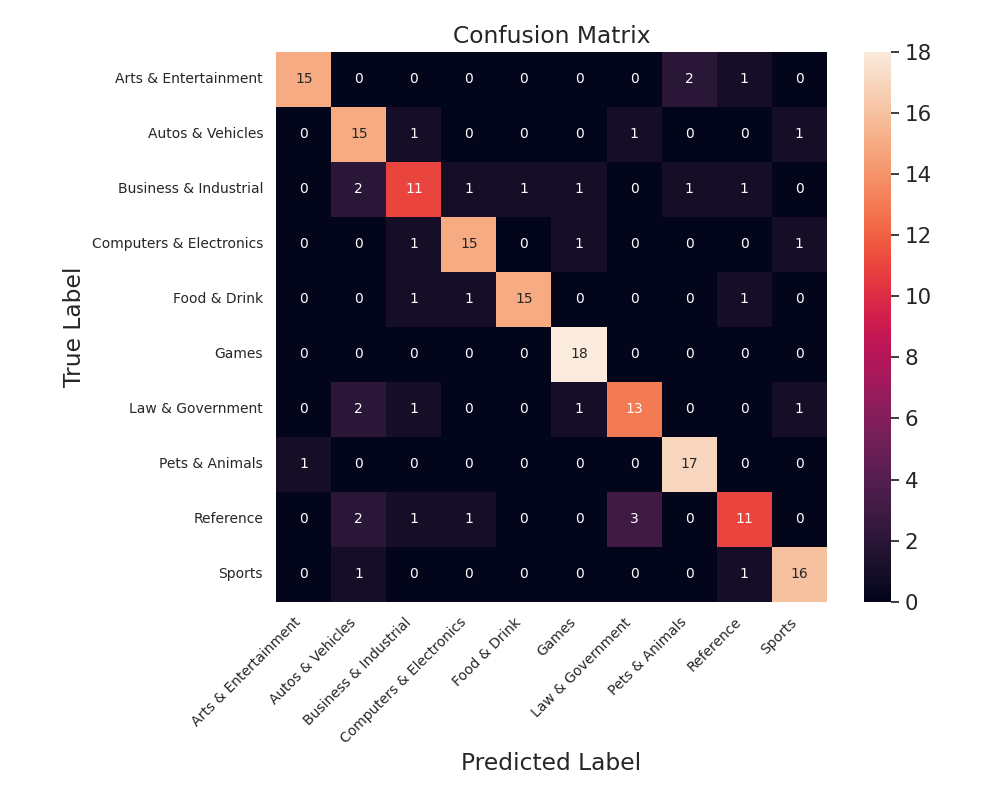
\includegraphics[width=0.8\linewidth]{asset/confusion_val.png} % Replace with actual image
\end{center}
   \caption{Confusion matrix of the 4 layers(MLP) model on the test set.}
\label{fig:confusion_matrix}
\end{figure}

%Our method achieves a compelling balance of high accuracy and drastically reduced training time, around 1 minute, compared to traditional complex models like 10 hours for TimeSformer fine-tuning.

The proposed methodology successfully achieves a compelling balance of high accuracy and significantly reduced training time, in comparison to conventional complex models such as TimeSformer fine-tuning, which can required up to ten hours.
\section{Conclusion}

%We have presented an efficient and effective approach for general video classification. Our key findings highlight that:

The paper sets out an efficient and effective approach for general video classification.

The following key findings are highlighted:

%\begin{itemize}
    %\item The proposed method significantly outperforms baselines in accuracy with a drastically reduced training time.
    %\item Integrating multimodal embeddings, particularly metadata embeddings derived from textual information, substantially enhances model performance.
    %\item Our novel data augmentation strategy applied in the embedding space is effective in mitigating overfitting and improving generalization.
    %\item A 4-layer MLP architecture provided the best trade-off between performance and complexity for our task.
%\end{itemize}

\begin{itemize}
    \item The proposed method demonstrates a substantial improvement in accuracy, accompanied by a significant reduction in training time.
    \item The integration of multimodal embeddings, notably metadata embeddings derived from textual information, has resulted in a substantial enhancement of model performance.
    \item The novel data augmentation strategy applied in the embedding space has been proved to be effective in mitigating overfitting and enhancing model generalization capabilities.
    \item The 4-layer MLP architecture was determined to provide the optimal trade-off between performance and complexity for the task at hand.
\end{itemize}

%This work demonstrates the potential of using carefully chosen pre-trained embeddings and systematic ablation studies to design lightweight yet powerful video classification models.

%While our method outperformed all baseline approaches on the evaluated tasks, it was only validated on a small subset of YouTube-8M. For a more comprehensive assessment and future work, it should be applied to larger-scale datasets such as Kinetics or the full YouTube-8M dataset.
% mention about limitations

This work demonstrates the potential of using carefully chosen pre-trained embeddings and systematic ablation studies to design a lightweight, yet powerful, video classification models. 

While the proposed methodology outperformed all baseline approaches on the evaluated tasks, it should be noted that validation was undertaken on a small subset of YouTube-8M.
For a more comprehensive assessment and future work, it should be applied to larger-scale datasets such as Kinetics or the original YouTube-8M dataset.

\newpage
{
    \small
    \bibliographystyle{ieeenat_fullname}
    \bibliography{main}
}

% WARNING: do not forget to delete the supplementary pages from your submission 
% \clearpage
\setcounter{page}{1}
\maketitlesupplementary


\section{Rationale}
\label{sec:rationale}
% 
Having the supplementary compiled together with the main paper means that:
% 
\begin{itemize}
\item The supplementary can back-reference sections of the main paper, for example, we can refer to \cref{sec:intro};
\item The main paper can forward reference sub-sections within the supplementary explicitly (e.g. referring to a particular experiment); 
\item When submitted to arXiv, the supplementary will already included at the end of the paper.
\end{itemize}
% 
To split the supplementary pages from the main paper, you can use \href{https://support.apple.com/en-ca/guide/preview/prvw11793/mac#:~:text=Delete%20a%20page%20from%20a,or%20choose%20Edit%20%3E%20Delete).}{Preview (on macOS)}, \href{https://www.adobe.com/acrobat/how-to/delete-pages-from-pdf.html#:~:text=Choose%20%E2%80%9CTools%E2%80%9D%20%3E%20%E2%80%9COrganize,or%20pages%20from%20the%20file.}{Adobe Acrobat} (on all OSs), as well as \href{https://superuser.com/questions/517986/is-it-possible-to-delete-some-pages-of-a-pdf-document}{command line tools}.

\end{document}
